\chapter{系统实现}

\section{开发环境的创建}
App端:本项目的App端和服务器端采用JavaScript语言进行开发,App端使用微信开发者工具作为开发环境,微信开发者工具是一个可以模拟微信客户端表现的开发和调试工具;
\par
识别模块:识别模块采用python语言开发,版本为3.6.8,开发环境是PyCharm;
\par
服务端:服务端使用Nginx作为web服务器,JavaScript的运行环境是Node.js,开发环境是WebStorm,使用的数据库是MySQL 8.0.13。本项目部署在腾讯云学生机上进行运行和测试,具体配置信息为一颗核心处理器,2G内存,1Mbps带宽,50GB系统盘,公共镜像为CentOS 7.2。

\section{账号功能的实现}
\subsection{登陆功能}
用户输入用户名和密码后通过表单提交给服务器,如果提交失败App端会提示用户检查是否为本机网络连接问题,如果提交成功服务端在收到网络请求后,在数据库中查询用户是否存在和用户的密码,把表单提交的密码与从数据库取出的密码比较后确定密码是否正确,把比较结果发送给App端。App端根据收到的结果决定是否让用户登陆。如果用户名和密码匹配,在服务端生成新的session,http响应把用户角色返回给客户端。
\par
小程序没有cookie机制,需要自行实现cookie来保持客户端和服务端的连接,session存储在服务器上,cookie有效期设为1800秒,客户端收到http响应后把响应头中的set-cookie取出,赋值到全局变量中,添加到后面每次http请求的请求头中,用来保持连接,确定是那个用户的操作。
\begin{figure}[h!]
	\centering
	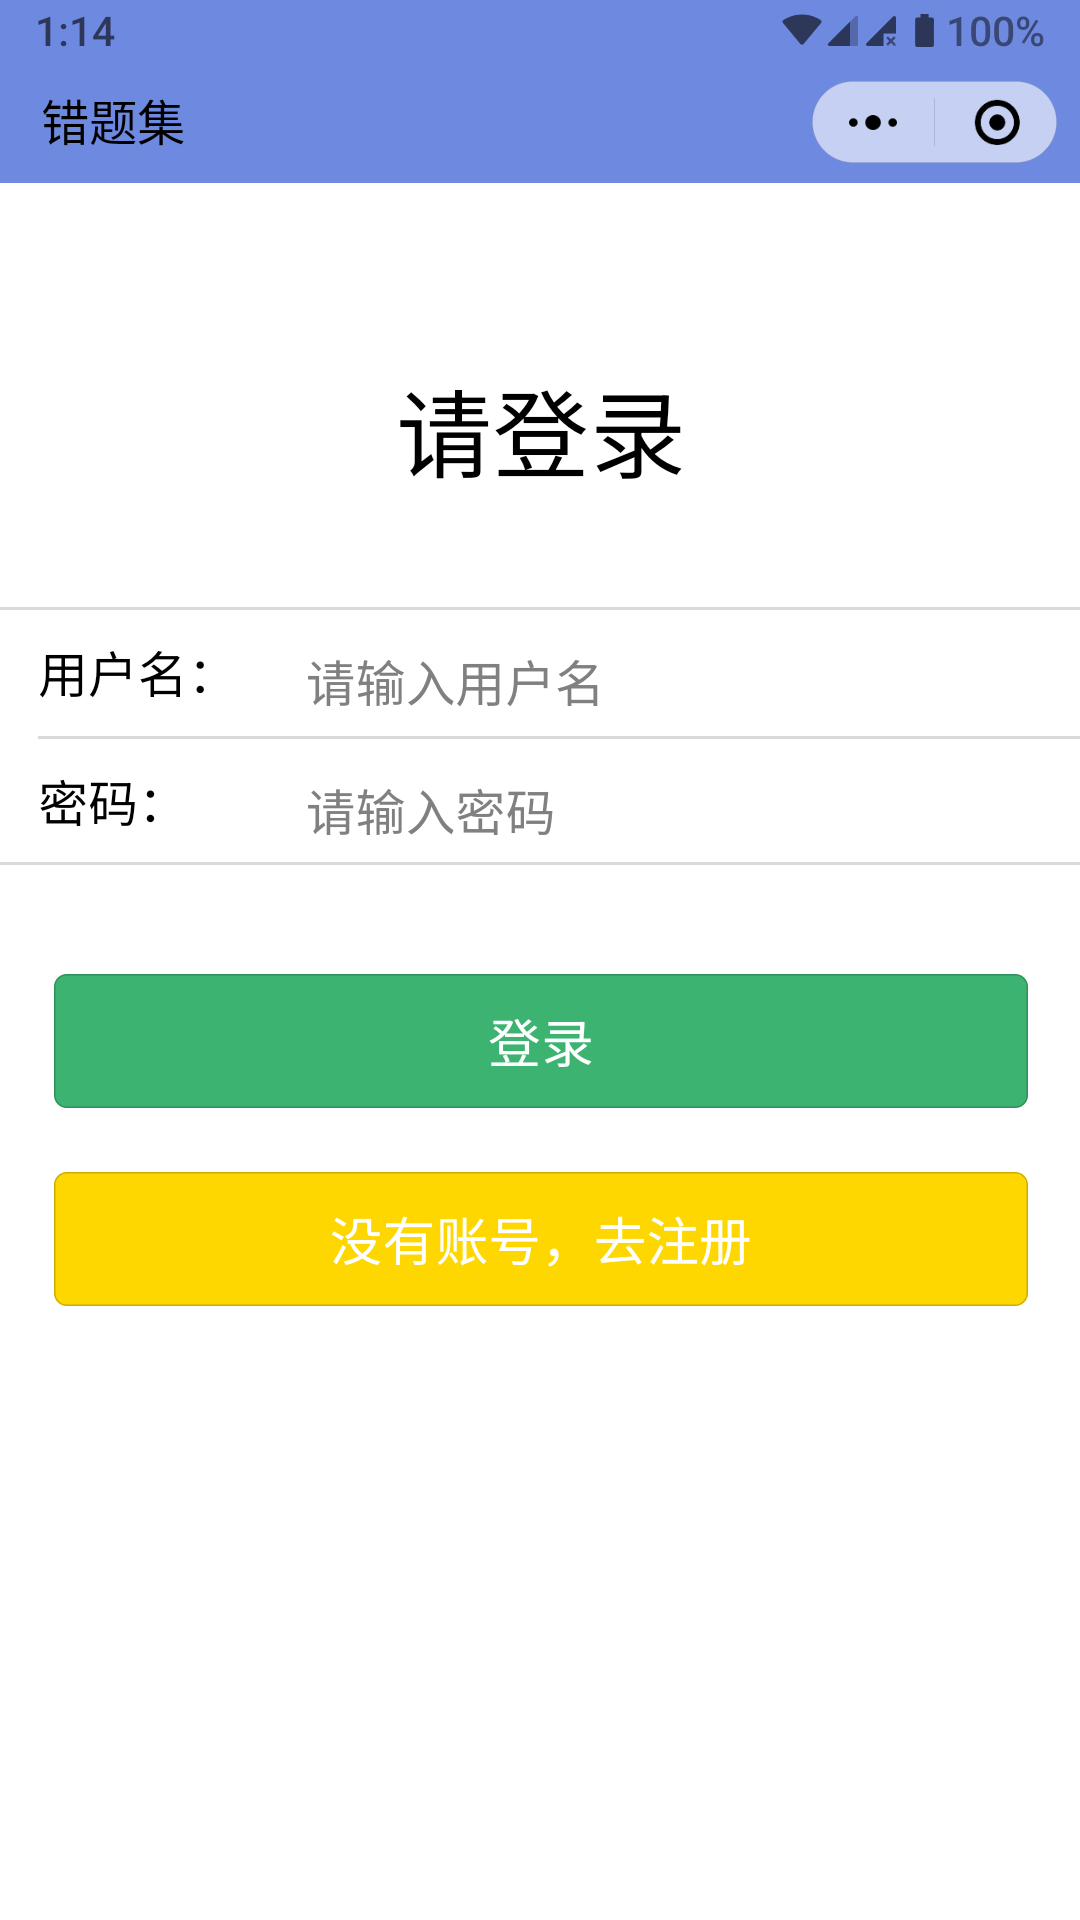
\includegraphics[width=108bp, height = 192bp]{picture/login.png}
	\caption{登陆界面}
	\label{fig:}
\end{figure}
\newpage
\subsection{注册功能}
App端把用户填写的表单提交给服务器,表单提交的数据包括用户名、用户角色、电子邮箱地址和登陆密码,服务器收到表单内容后把用户添加到数据库中,每个用户的用户名是唯一的,所以在用户填写表单时要查询该用户名是否已被使用,如果用户名已经被占用、两次输入的密码不一致或表单未完全填写,会分别提示用户该名称已经被占用、密码与确认密码不一致和信息填写不完整,并且用户无法提交数据。注册成功后会跳转到用户登陆界面。

\begin{figure}[h!]
	\centering
	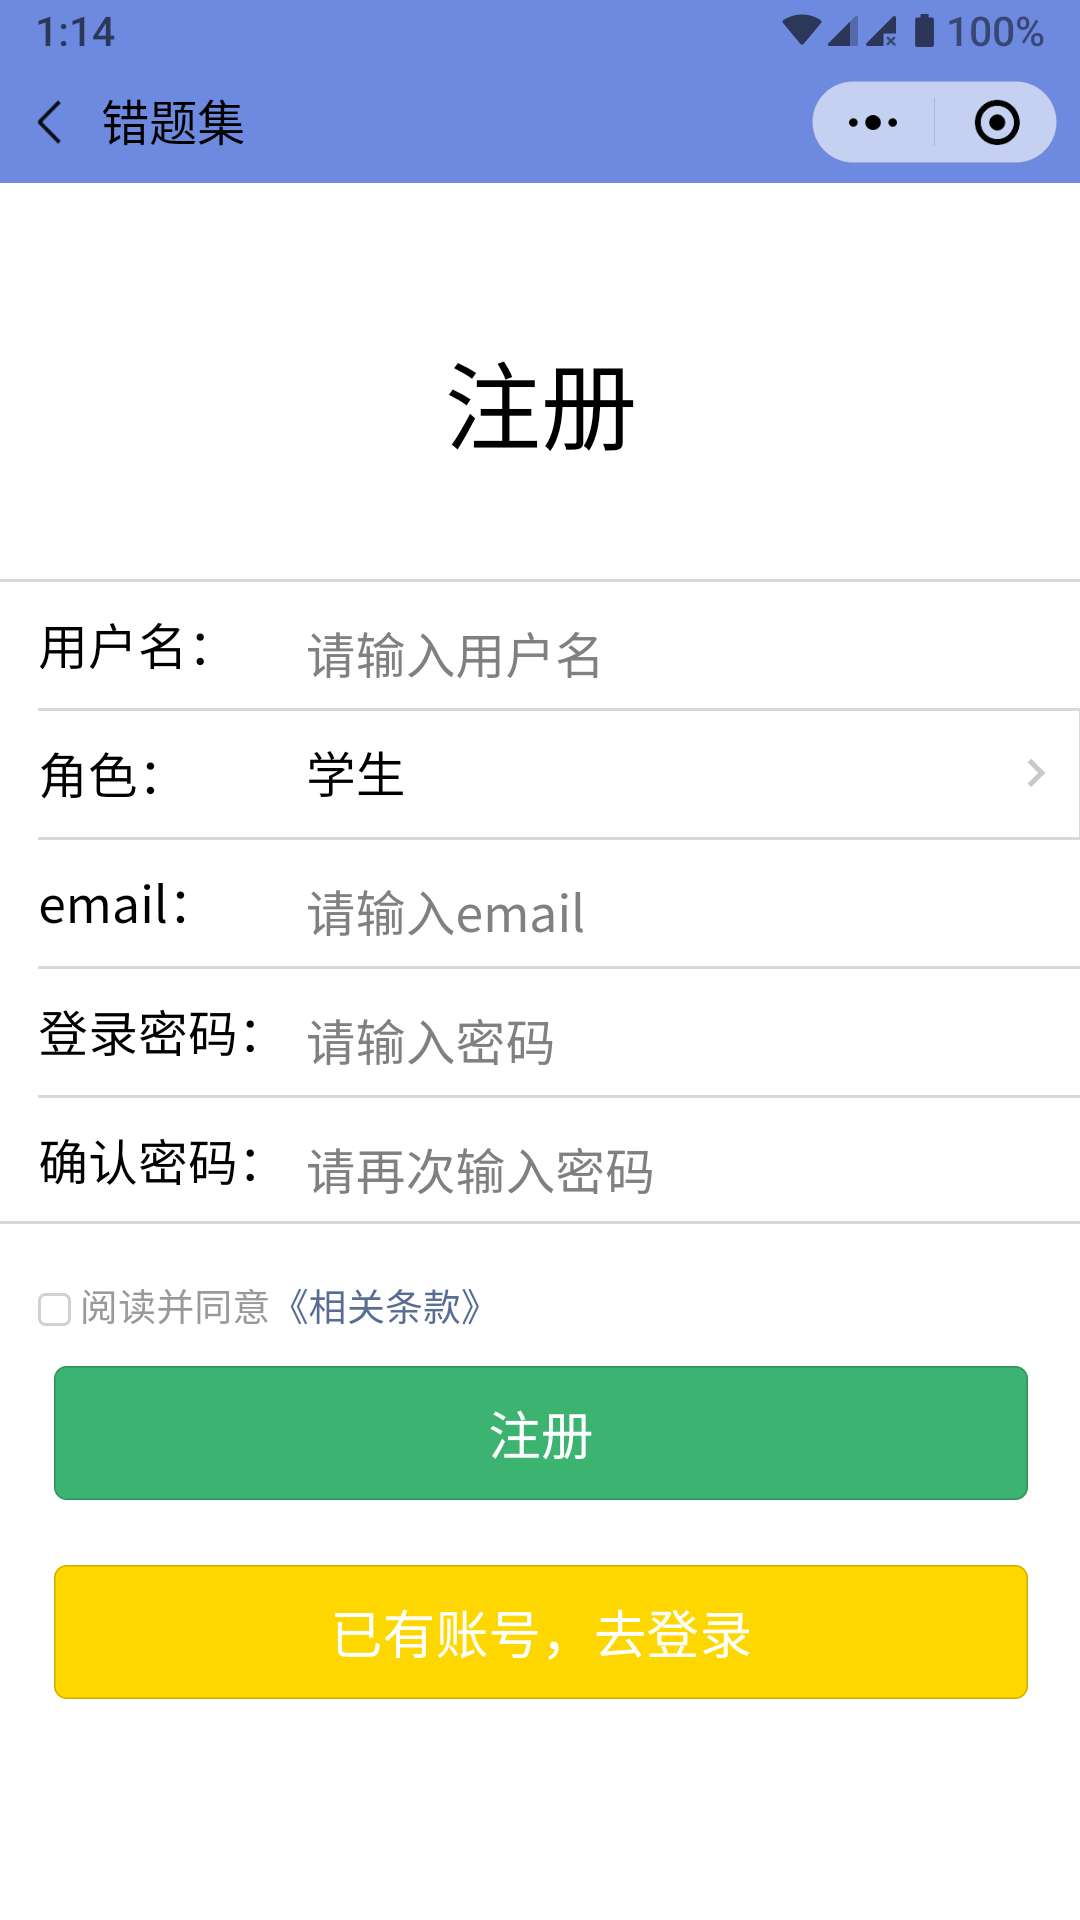
\includegraphics[width=108bp, height = 192bp]{picture/register.jpg}
	\caption{注册界面}
	\label{fig:}
\end{figure}
\newpage

\subsection{管理员功能的实现}
查看用户:管理员可以看到所有用户和他们的角色以及所在班级。点击查看用户按钮后客户端会向服务端发送查询请求,服务端返回所有用户的用户名、角色和班级,客户端收到响应后把数据以特定的样式呈现给管理员。
\par
添加用户和注册类似,按要求填写好数据后,提交表单后服务端把相应的信息写进数据库就完成了添加用户,如果用户名已存在或两次输入密码不一致或未填写完整,会分别提示用户名已被使用、输入密码不一致和请把信息填写完整。
\par
删除用户只需填写要删除的用户名,服务端接受请求后将数据库中用户名为请求中用户名的记录全部删除,删除用户就完成了。如果用户名不存在或者未填写用户名会弹出相应的提示,点击删除用户按钮会弹出确认窗口防止用户错误操作。
\begin{figure}[h!]
	\centering
	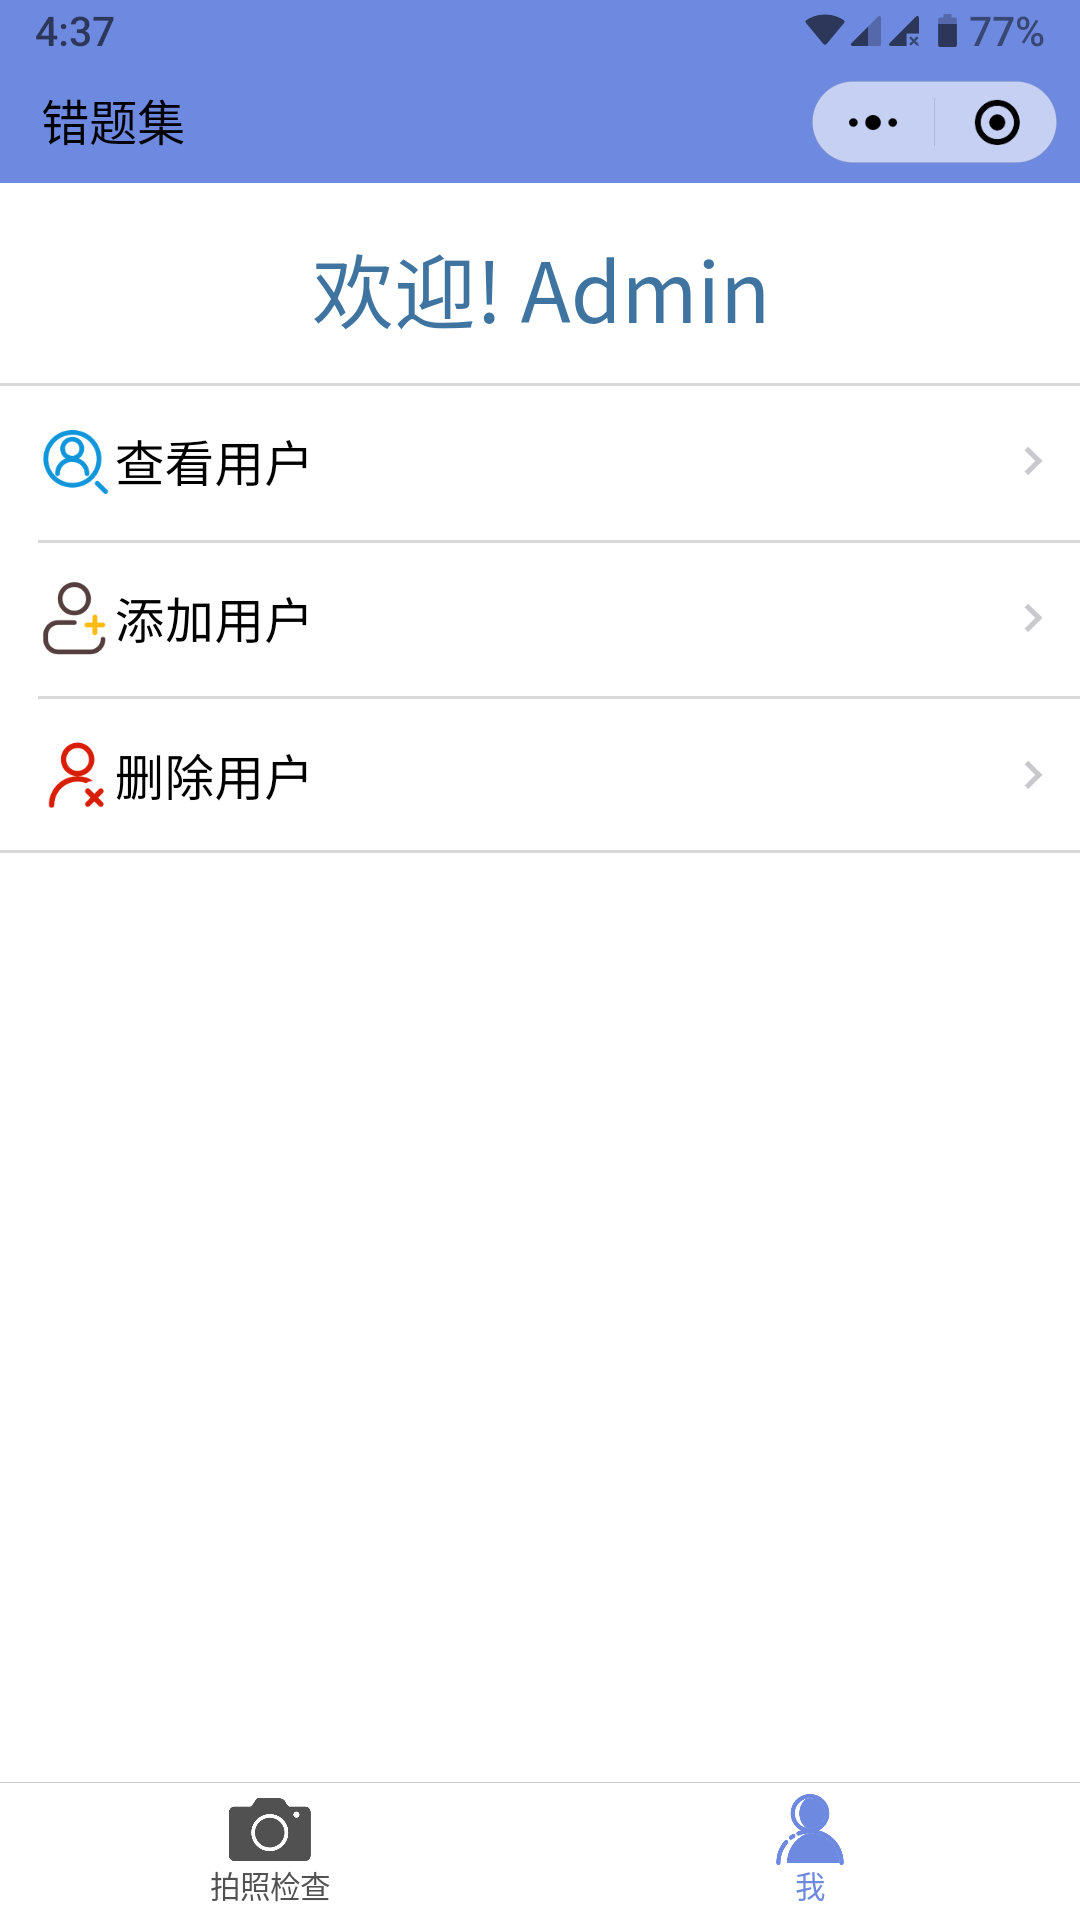
\includegraphics[width=108bp, height = 192bp]{picture/admin.png}
	\caption{管理员界面}
	\label{fig:}
\end{figure}
\newpage

\subsection{识别算式功能的实现}
识别算式模块主要功能是把图片上传到服务器,服务器收到用户检查请求后开启子进程执行识别程序,识别和检测程序检测图片中的算式之后,把结果标记在图片上,并把检查获得的数据存储到数据库,最后通过http响应以json或字符串的形式把结果图片的url发送给App端。App端通过http请求获取数据后,通过数据绑定把图片呈现在视图层。
\begin{figure}[h!]
	\centering
	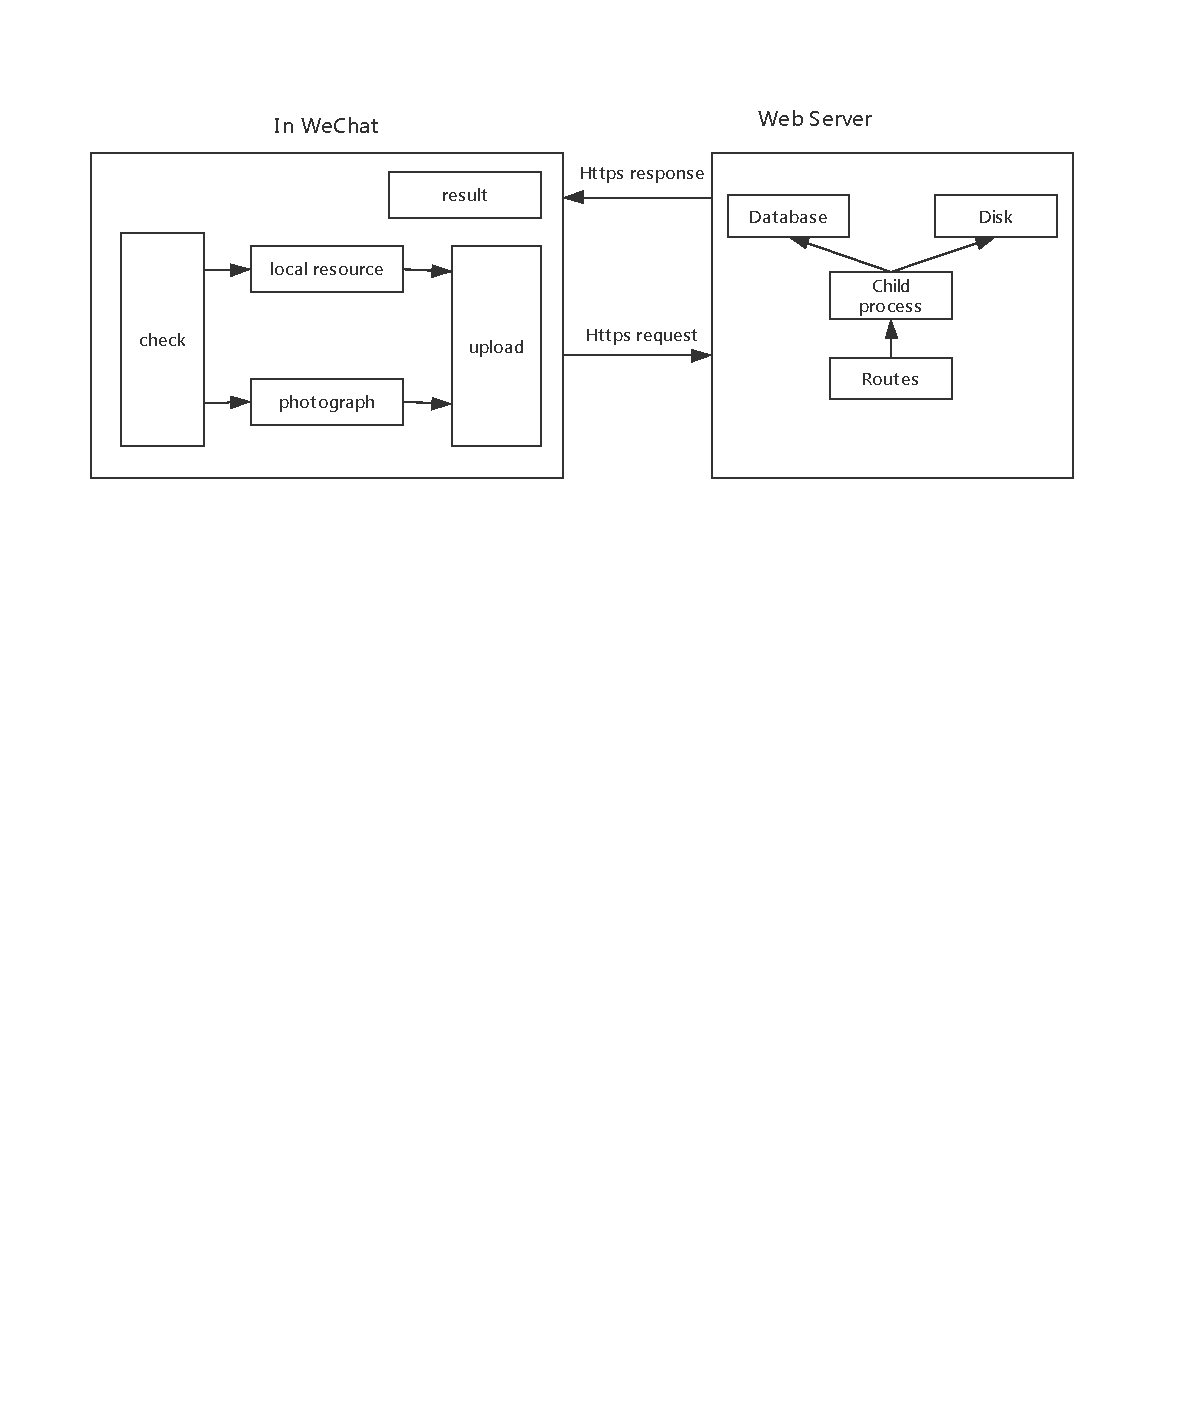
\includegraphics[width=350bp]{picture/identify.pdf}
	\caption{识别过程}
	\label{fig:}
\end{figure}
\par

\subsubsection{App端上传图片和展示结果}
拍照和从相册中选择是上传图片的两种来源,可以点击相机图标打开摄像头拍照,或者从相册中选择图片。
\begin{figure}[h!]
	\centering
	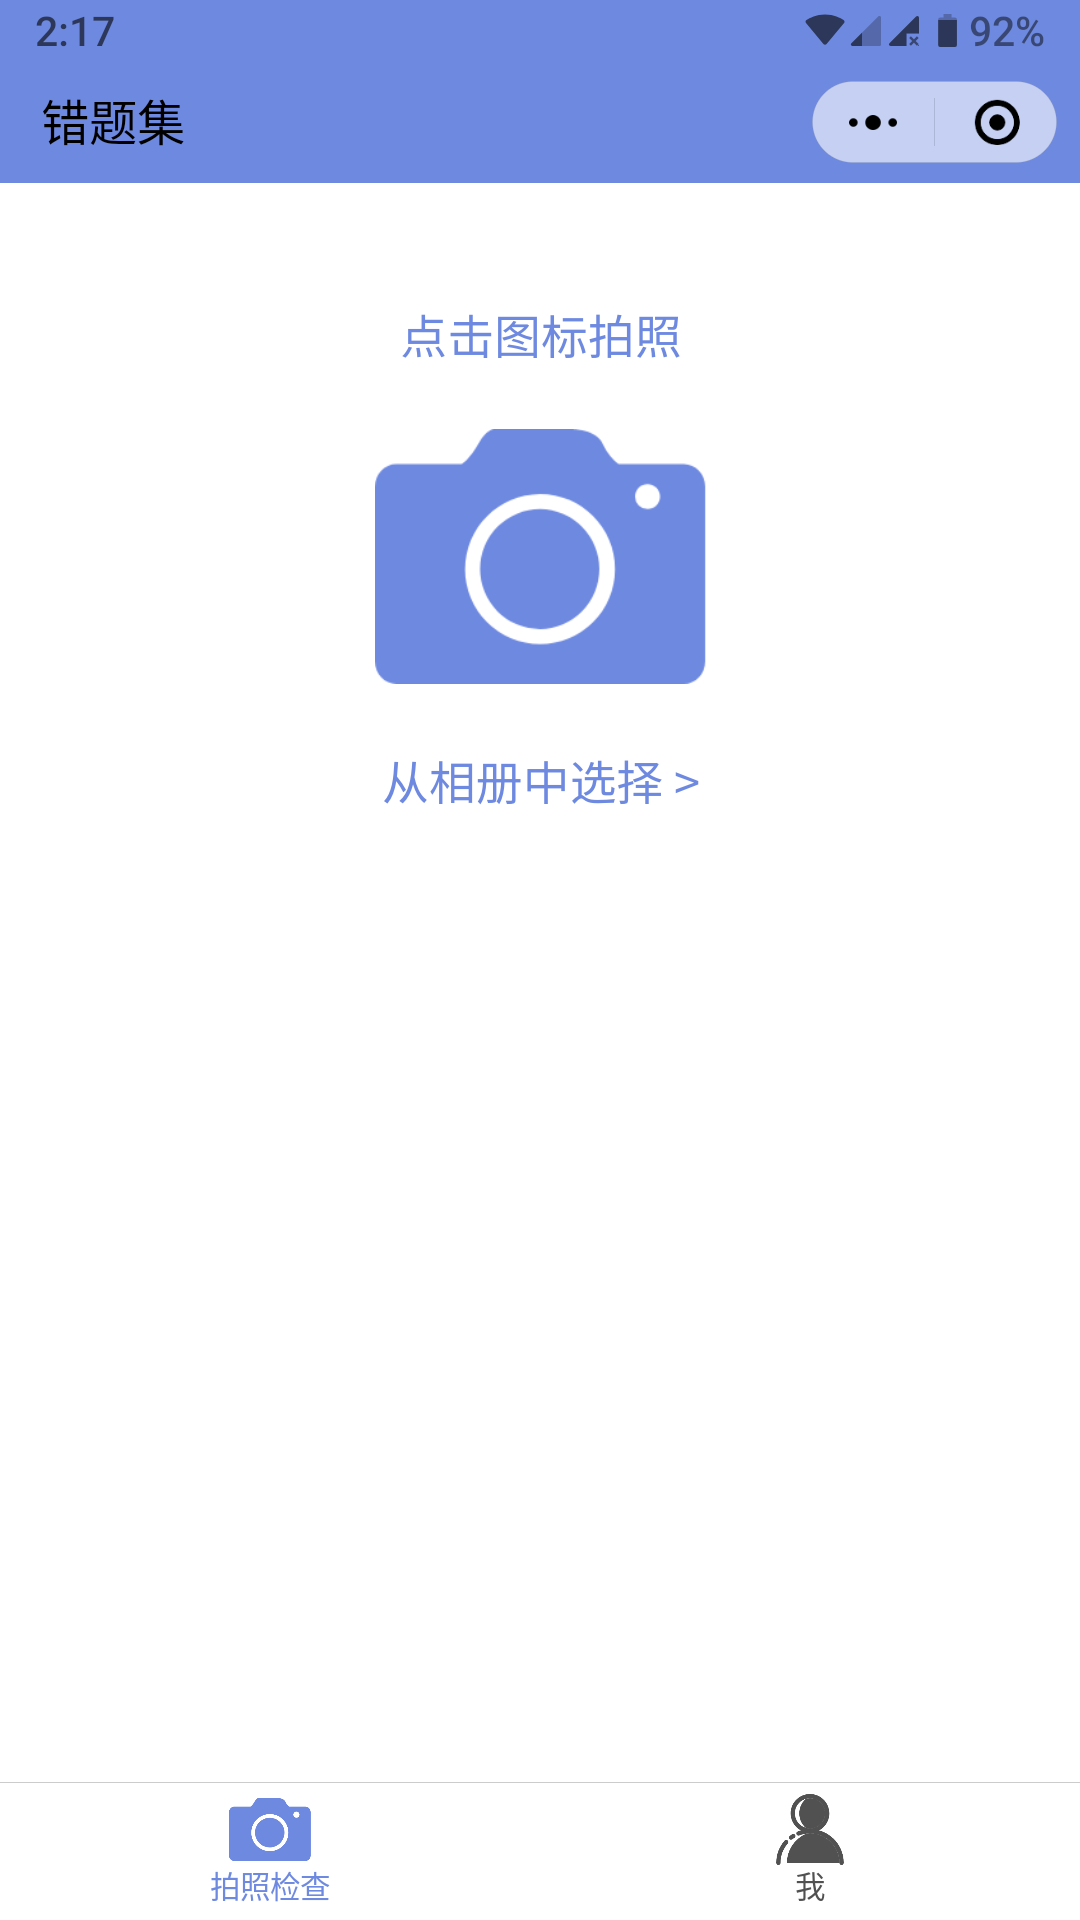
\includegraphics[width=108bp, height = 192bp]{picture/check.png}
	\caption{识别算式界面}
	\label{fig:}
\end{figure}
\newpage
使用ctx.takePhoto调用摄像头拍摄图片,然后使用wx.chooseImage和wx.uploadFile把图片上传到服务器上的临时目录;完成图片上传后会跳转到结果界面,结果界面通过http请求获取检查结果图片的url,在页面完成初次渲染时把结果呈现在视图层。
\begin{figure}[h!]
	\centering
	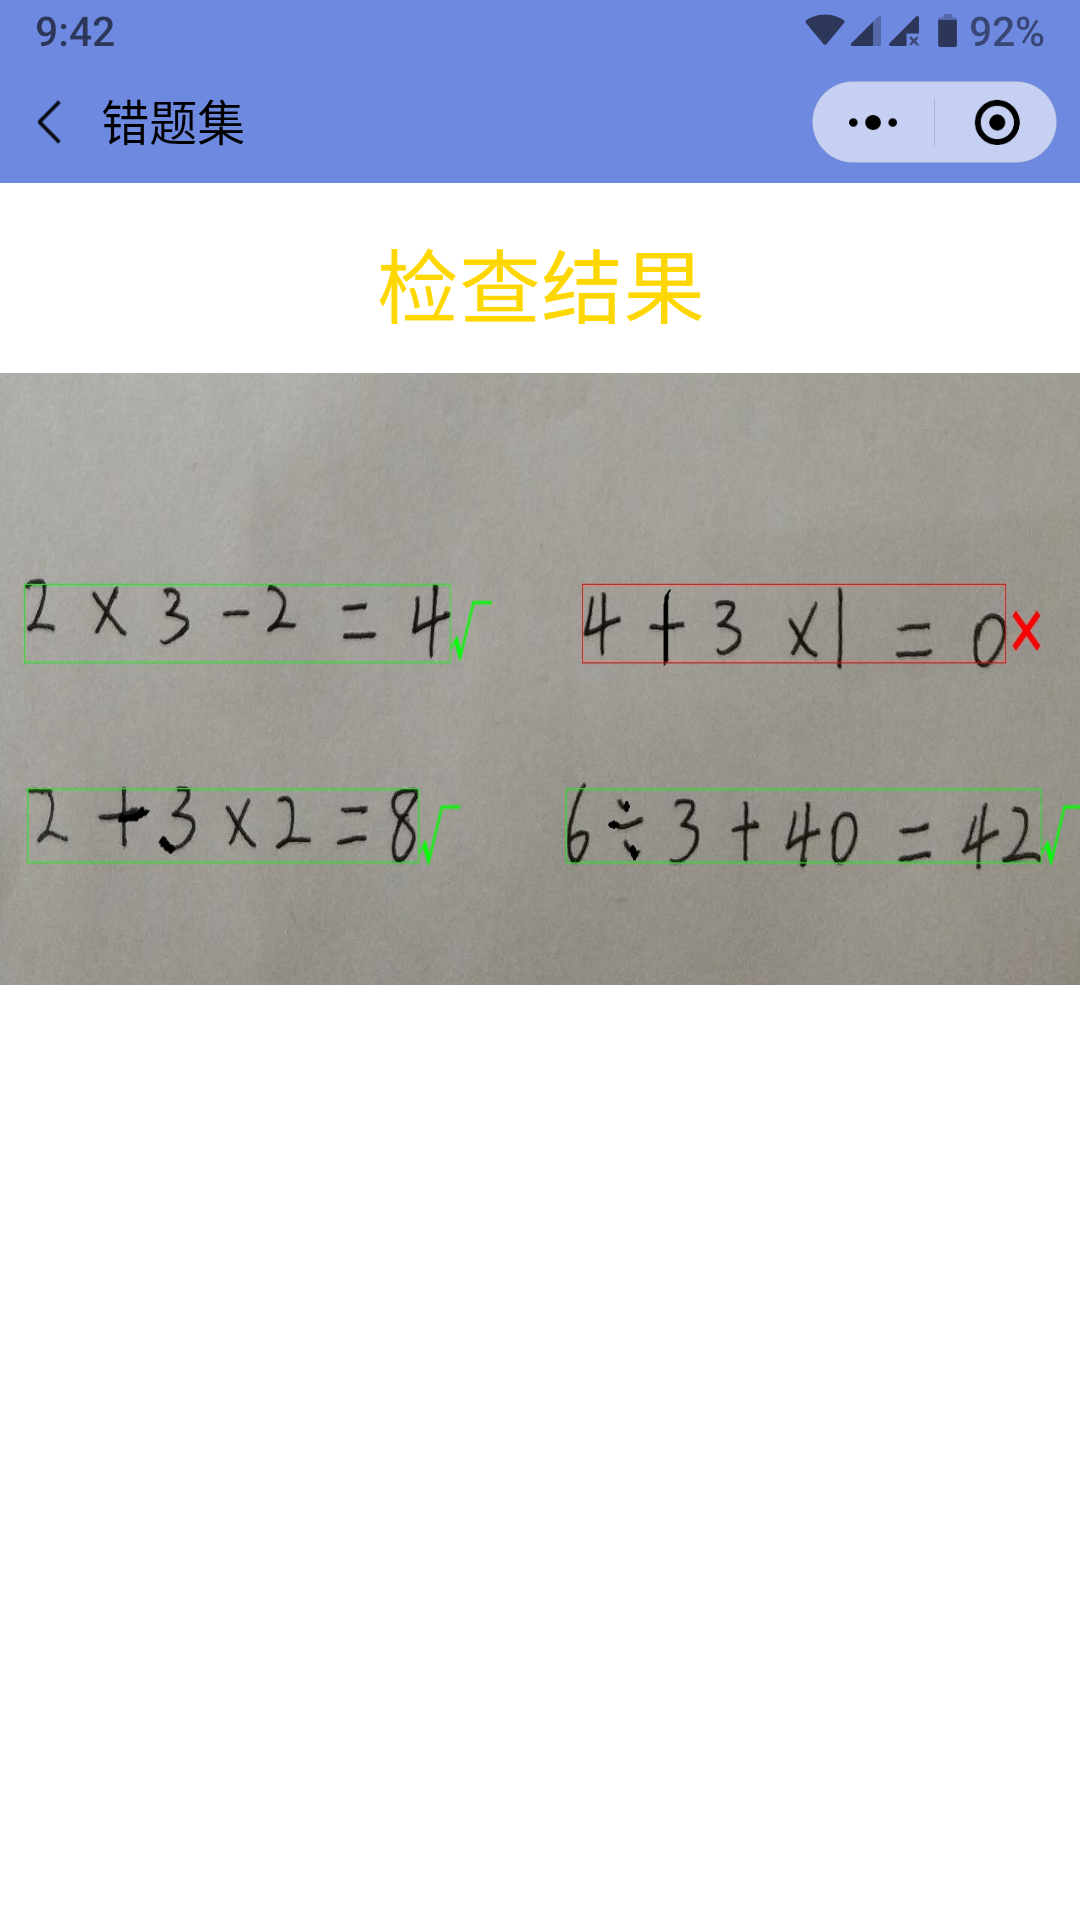
\includegraphics[width=108bp, height = 192bp]{picture/result.png}
	\caption{识别结果界面}
	\label{fig:}
\end{figure}
\par

\subsubsection{服务端处理图片}
服务端是一个Node.js Express项目,通过Multer中间件获取上传的文件,并将它们存储在硬盘中。同时创建子进程来调用处理图片的python程序,使用python命令行参数来输入图片路径和产生结果路径,python程序获得图片输入后,首先进行转灰度图、二值化,然后统计字符像素的直方图,选取合适的阈值切分算式,同时标记每个字符在图片中的位置和算式的序号,方便后面标记结果。把切分好的图片填充和调整到28*28的大小后输入到模型中识别,把识别的结果拼接成算式,判别是否正确,把结果标记在原图上,把结果图存在硬盘中,并打印出错的算式,父进程获得子进程的输出转化成字符串后,把这些数据存储到数据库中,最后产生json格式的http响应把结果图片的url传给

\subsection{错题集功能模块的实现}
学生在用户中心可以完善自己的个人信息,查看自己提交过的历史错题记录和对自己错题的统计分析以及相应错题的相关推荐。

\begin{figure}[h!]
	\centering
	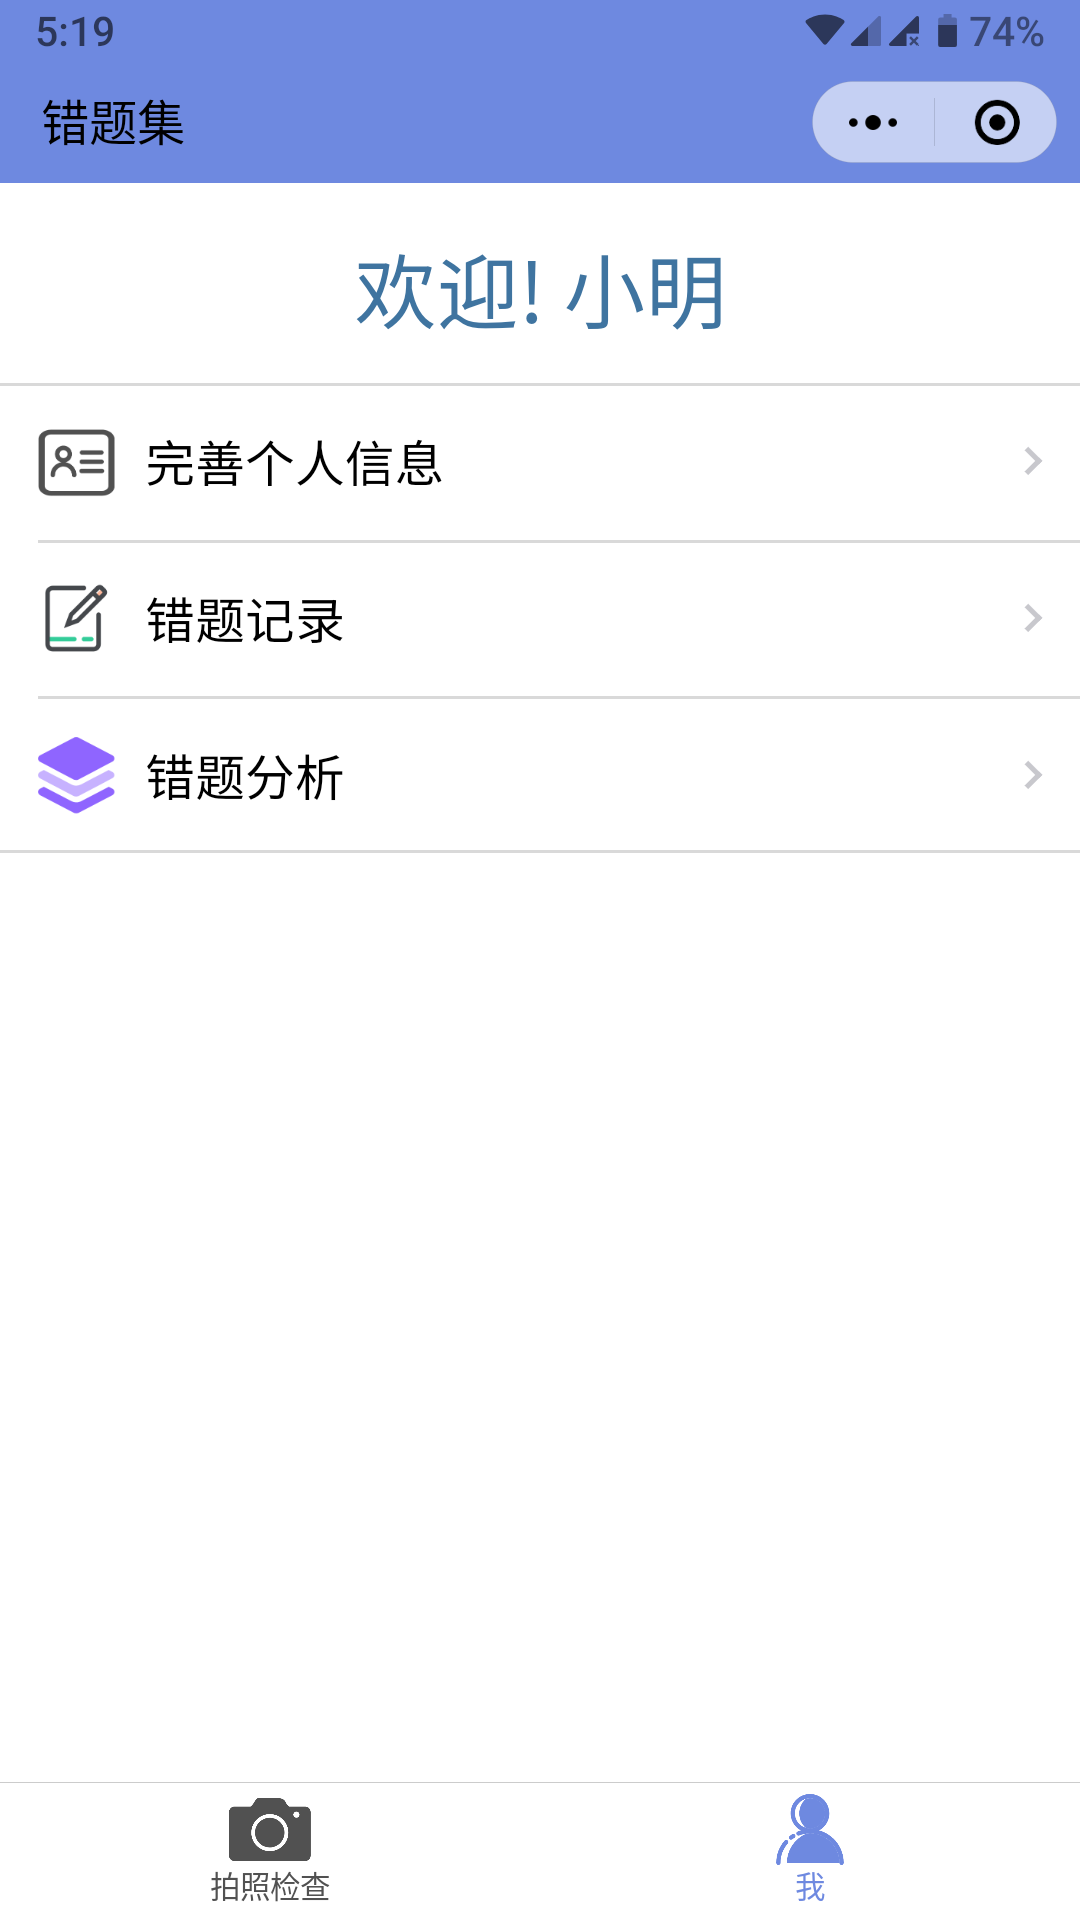
\includegraphics[width=108bp, height = 192bp]{picture/user.png}
	\caption{用户中心界面}
	\label{fig:}
\end{figure}
\newpage
查看检查的历史记录,点击错题记录后客户端发送查询历史记录请求,服务端收到请求后在数据库查询相应数据,然后通过响应把数据发送到客户端,客户端按照日期展示历史检查结果,点击图片后可以放大预览。

\par
统计自己出过错的算式,点击错题分析按钮发送查询请求,服务端查询该用户的出错题目和次。客户端收到结果后可以看到自己出错的题目和出错的次数,点击出错算式后的推荐链接后,服务端会根据用户名和算式计算出与该算式相关的其它算式,在跳转后的页面呈现给用户。
\begin{figure}[h!]
	\centering
	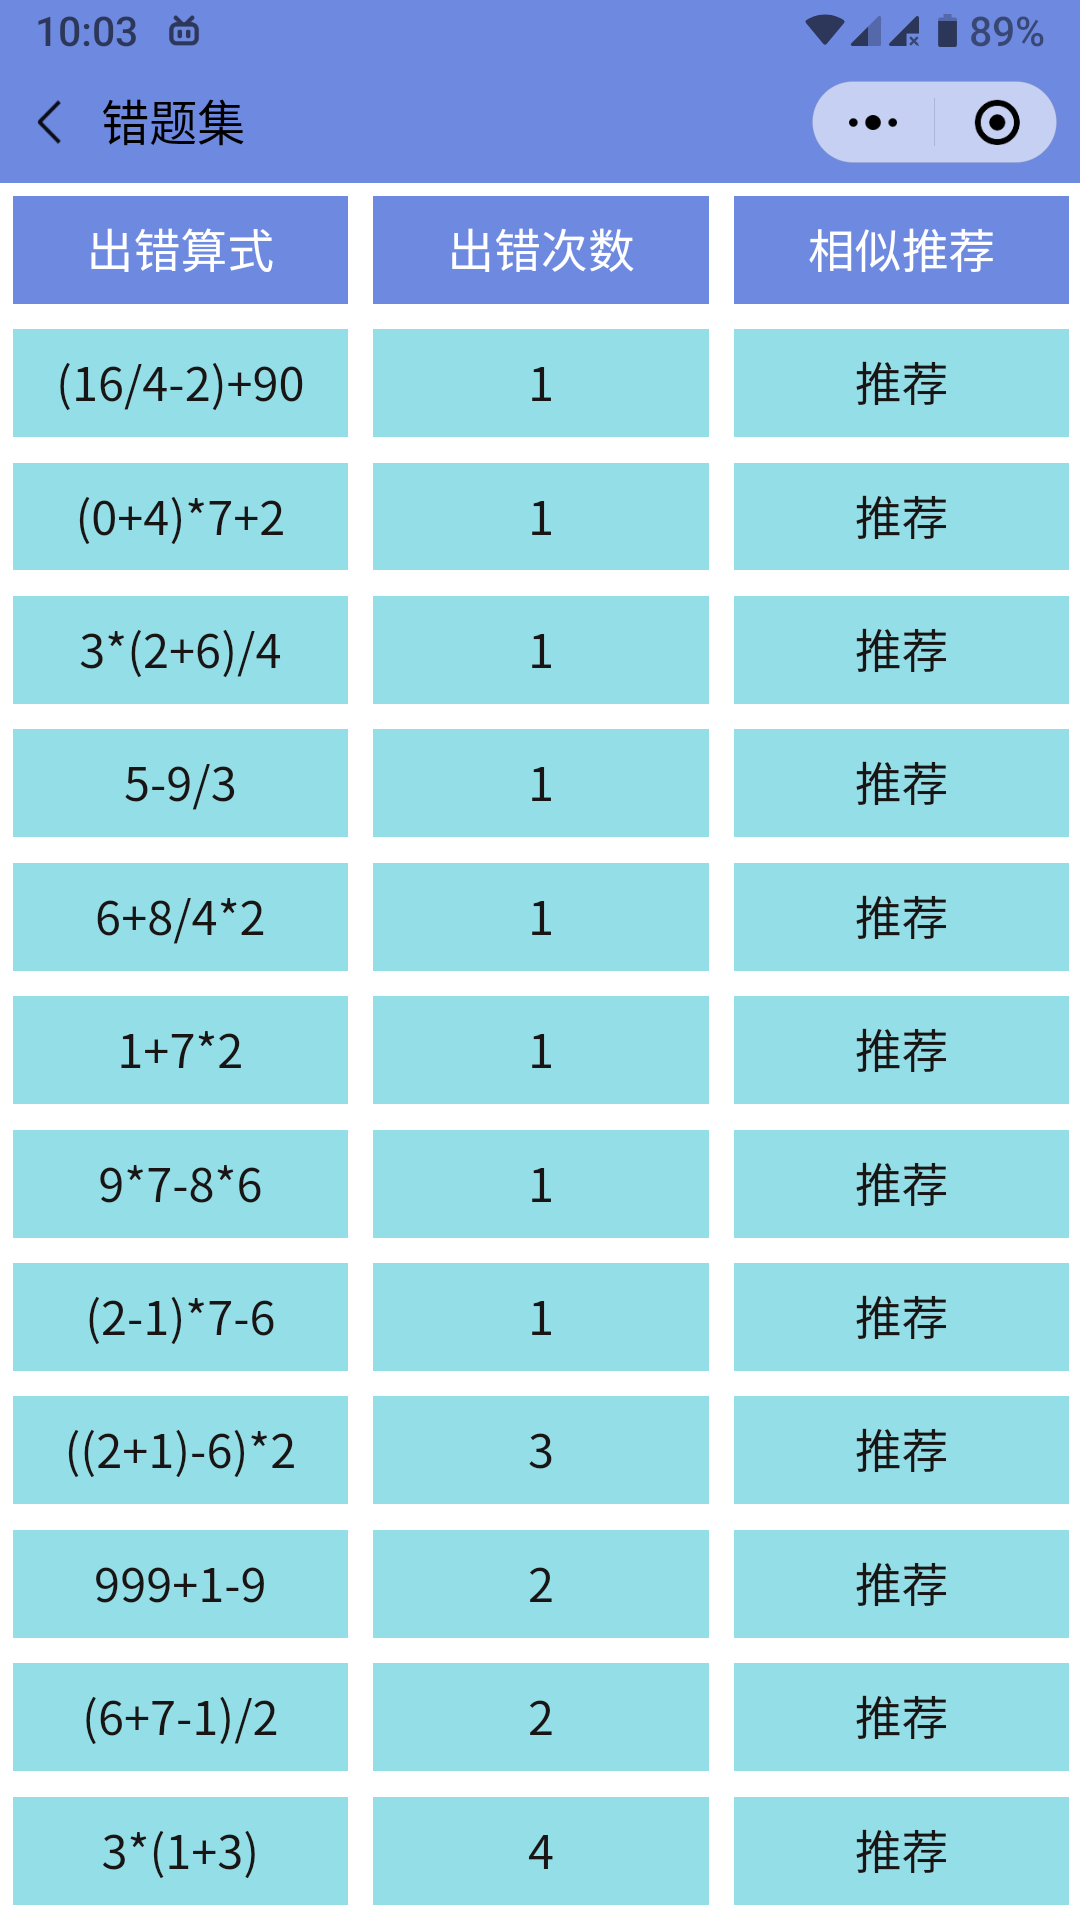
\includegraphics[width=108bp, height = 192bp]{picture/analysis.png}
	\caption{错题分析图}
	\label{fig:}
\end{figure}
\par
老师可以查看所有人的出错记录和对应的次数,角色为老师的用户在点击错题分析按钮后,会发送查询所有用户出错记录的请求,服务端鉴定完用户名和角色后查询对应的数据,然后把查询结果发送到客户端,客户端把查询结果呈现在视图层。
\begin{figure}[h!]
	\centering
	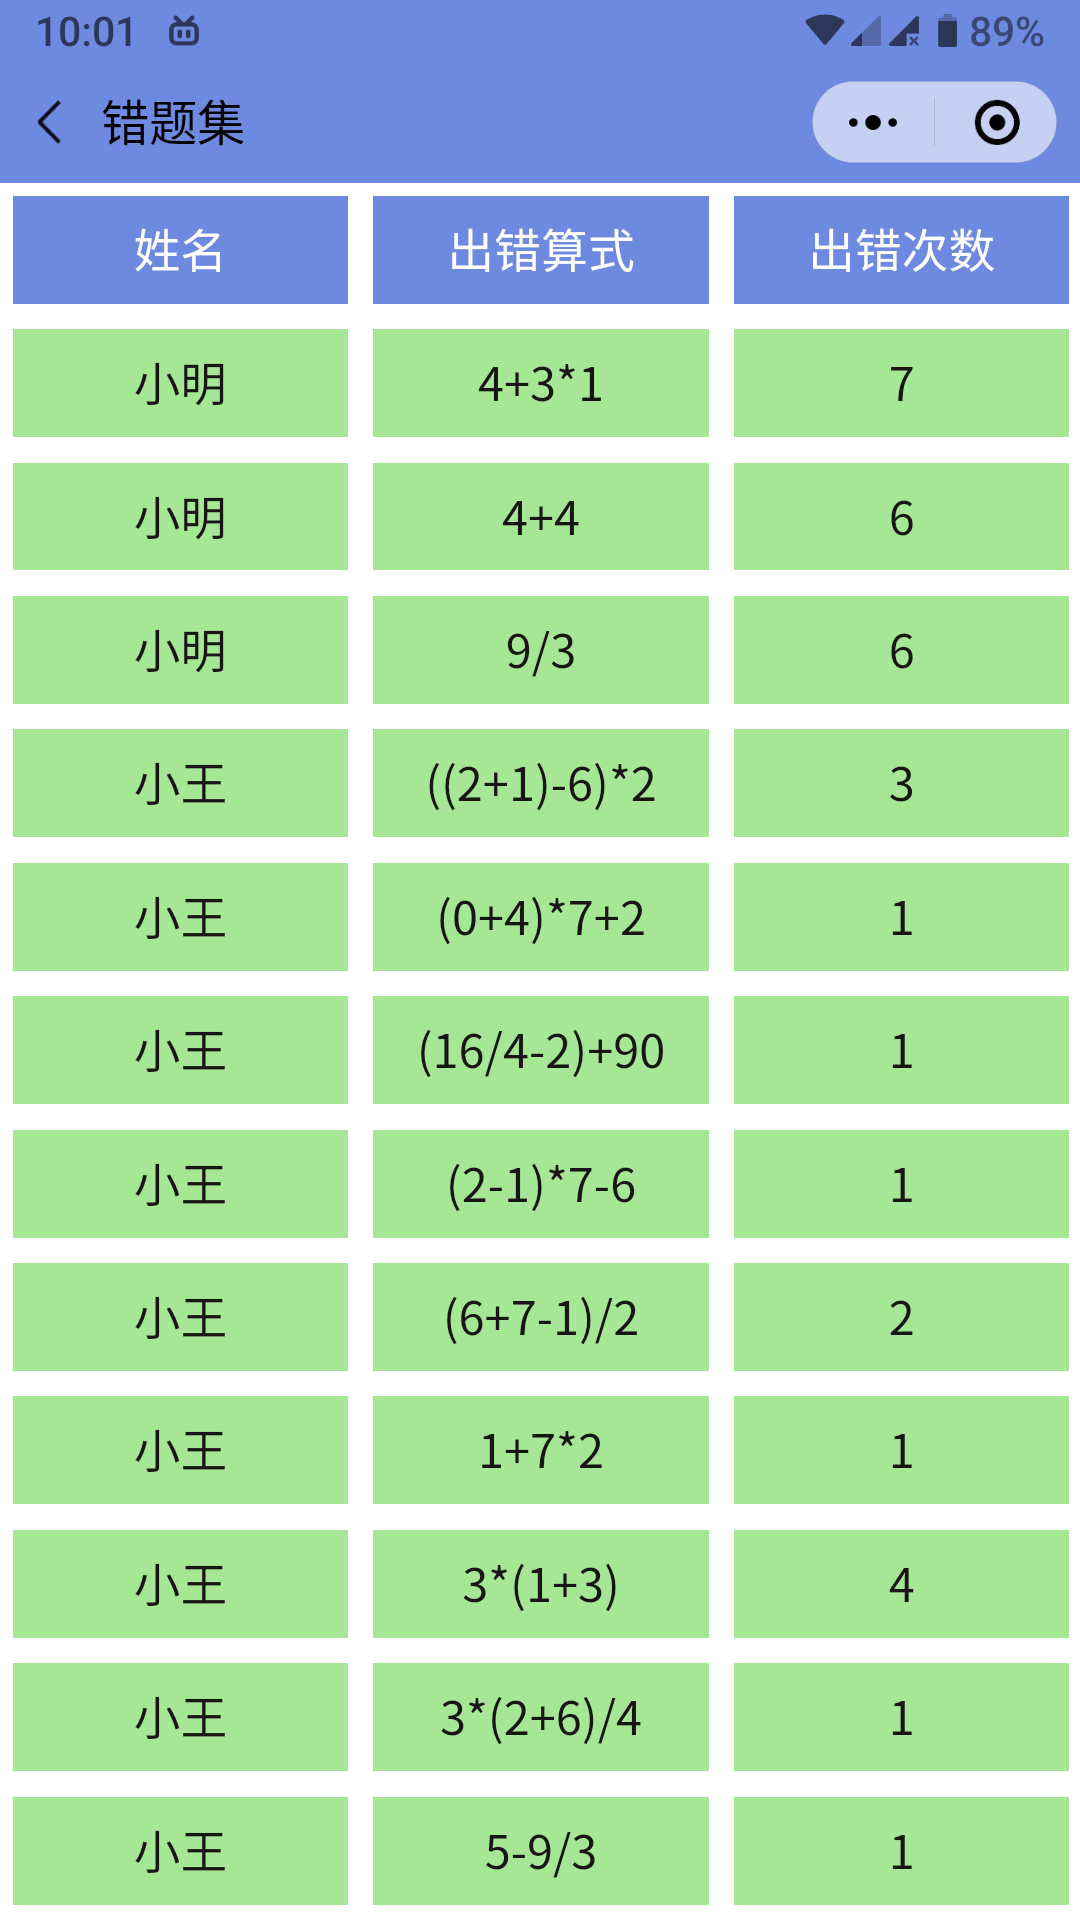
\includegraphics[width=108bp, height = 192bp]{picture/statistic.png}
	\caption{错题统计图}
	\label{fig:}
\end{figure}
\par
\section{基于协同过滤推荐算法实现相似算式推荐}
基于物品的协同过滤推荐算法预先根据所有用户对物品的评价计算出所有物品之间的相关性,然后把与此件物品最相关的物品推荐给用户。为了实现相似算式推荐,可以把用户做错该算式的次数作为用户对此道题的评价,使用所有用户做错算式的次数计算每两道算式间的皮尔逊相关系数。
\par
皮尔逊相关系数的计算公式:
\[ 
	r=\frac{\sum_{i=1}^n{(x_i-\bar{x})\cdot(y_i-\bar{y})}}
	{\sqrt{\sum_{i=1}^n{(x_i-\bar{x})}}\cdot\sqrt{\sum_{i=1}^n{(y_i-\bar{y})}}}
\]
\par
将算式按照皮尔逊系数排序,从高到低取出该用户未做的若干道算式,作为该道算式的推荐。也可以把该用户对几道算式的评分作为权重,加权排序后得到新的算式与出错算式的相关性。

\section{本章小结}

